\chapter{Luminescent Organic Materials}
\label{chapter: luminscent organic materials}
%%%%%%%%%%%%%%%%%%%%%%%%%%%%%%
\section{Introduction}\label{section: lom introduction}
Luminescent organic molecules have myriad of useful applications. In aqueous solution they are used extensively in biological imaging, probing, and detection. Deposited as thin films and aggregates, they represent the next generation of organic optoelectronics, where availability and low cost of starting materials, straightforward syntheses, and lightweight devices are attractive features. Perhaps most importantly, the luminescent response of molecular organic systems can be tuned with relative ease compared to their inorganic counterparts, emitting across the visible spectrum and producing white light. 

Since the discovery of electromluminescence in the 1960s, intensive efforts in academia and industry have delivered considerable progress in the field of organic electronics, leading to  the development of applications such as field-effect transistors, photovoltaic cells, optical memory devices, and single-crystal lasers.\cite{Ostroverkhova2016} The most prominent success story is certainly organic light-emitting diodes (OLEDs), which have already reached market adoption for lighting and display purposes. However, in many areas organic systems suffer from low efficiencies, trial-and-error optimisation, and decreased performance in aggregated form versus solution. 

To advance, there must be control over both the supermolecular structure of the material and the electronic structure of the  molecules within.  Unfortunately neither of these properties exist in isolation, and the interplay between them must also be intimately understood, which somewhat complicates matters. Of these three contributing factors, it is the relationship between the electronic structure and the environment which are of interest in this work. The luminescent response of molecules can change drastically from one medium to another, whether in the gas phase, as a solution, aggregated as clusters, or in molecular crystals. Understanding the interplay between the luminophore and its environment is crucial for designing more efficient materials from first principles. 

To this end, we approach this problem using theoretical chemistry methods to investigate organic compounds exhibiting aggregation induced emission (AIE).  AIE-active compounds are non-emissive in dispersed media, but undergo a switch-on of luminescence, typically in the form of fluorescence, upon aggregation. Since organic electronics are manufactured using a solid-state layer, AIE has attracted considerable interest as a pathway to overcome the common effect of aggregation caused quenching (ACQ), hitherto a major obstacle in the development of organic luminophores. In this chapter the problem of ACQ shall be introduced, followed by an examination of the AIE phenomenon through analysis of typical structures, mechanistic interpretations, and how quantum chemical methods are applied to model such systems.
%%%%%%%%%%%%%%%%%%%%%%%%%%%%%%
\section{Aggregation Caused Quenching}\label{section: lom ACQ}
Conventional photoinduced luminescence occurs after chromophores with $\pi$-conjugation absorb light in the UV/Vis region of the electromagnetic spectrum. In gas phase, fluorescence usually follows. In solution, the fluorescence is typically concentration dependent, undergoing a quenching as solute concentration is increased. In 1954, photochemisty pioneer  F\"{o}rster and Kasper elegantly showed how the fluorscence of pyrene is shifted and weakened with increasing concentration (Figure \ref{figure: Forster_Spectra}).\cite{Forster1954,Forster1969} As the concentration increases, a new fluorescent species is formed and the monomer fluorescence is decreased. The new band at lower energy is a result of the formation of excited dimers, or \textit{excimers}.
\begin{figure}[H]
\centering
  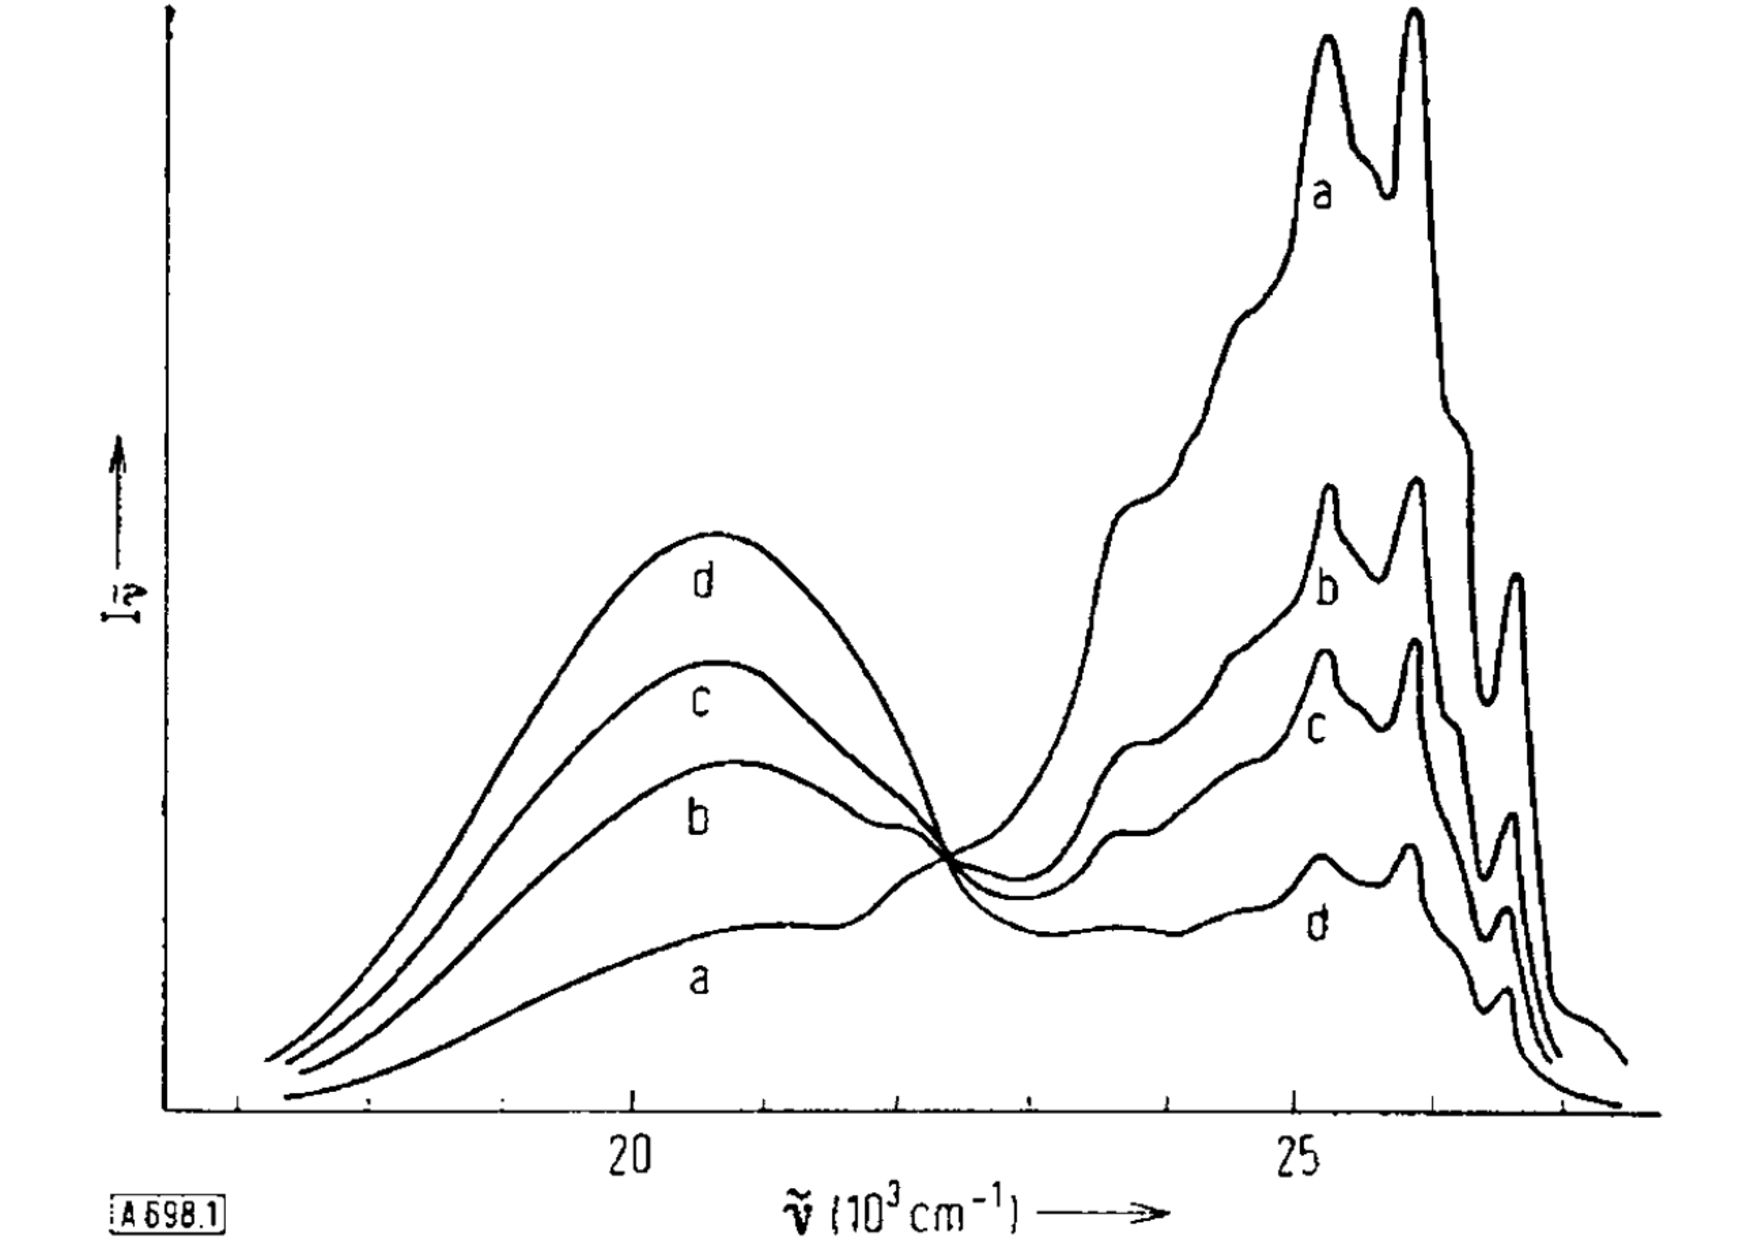
\includegraphics[width=0.6\linewidth]{Intro/Forster_Spectra.pdf}
  \caption{Fluorescence spectrum of pyrene (in n-heptane, 20 8C) at different concentrations: a) \SI{5.0e-5}, b) \SI{1.8e-4}, c) \SI{3.1e-4}, d) \SI{7.0e-4}{molL^{-1}}. Reproduced from ref.{~\citenum{Forster1969}} with permission of Wiley-VCH.}
  \label{figure: Forster_Spectra}
\end{figure}